\subsection{A Concise Introduction to Parallelism}
\makesubcontentsslidessec


\begin{frame}
  \begin{block}{Parallelism}\pause
    \begin{center}
    \begin{minipage}{.46\textwidth}
    \begin{block}{\centering Serial Programming}
      \begin{center}
      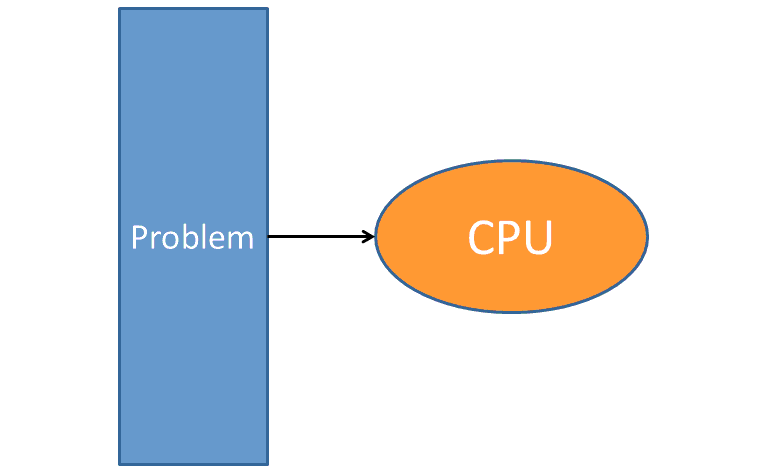
\includegraphics[width=.975\textwidth]{../common/pics/parallelism1}
      \end{center}
      \end{block}
    \end{minipage}
    \hspace{.15cm}
    \begin{minipage}{.46\textwidth}
    \begin{block}{\centering Parallel Programming}
      \begin{center}
      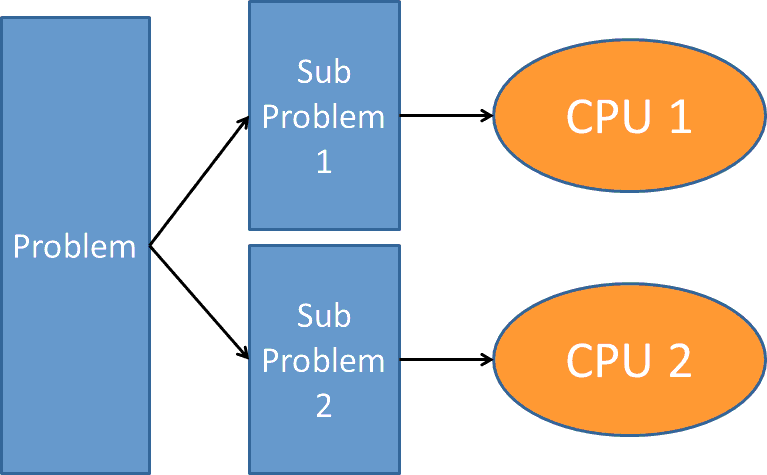
\includegraphics[width=.975\textwidth]{../common/pics/parallelism2}
      \end{center}
      \end{block}
    \end{minipage}
    \end{center}
  \end{block}
\end{frame}

\begin{frame}
  \begin{block}{Parallelism}\pause
    \begin{center}
    \begin{minipage}[t]{.46\textwidth}
    \vspace{0pt}
    \begin{block}{Serial Programming}
      \begin{center}
      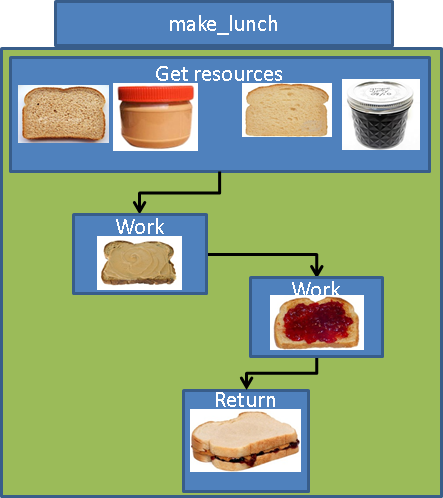
\includegraphics[width=.975\textwidth]{../common/pics/analogy_serial}
      \end{center}
      \end{block}
    \end{minipage}
    \hspace{.15cm}
    \begin{minipage}[t]{.46\textwidth}
    \vspace{0pt}
    \begin{block}{Parallel Programming}
      \begin{center}
    \includegraphics[height=5.45cm,width=.975\textwidth]%
    {../common/pics/analogy_parallel}
      \end{center}
      \end{block}
    \end{minipage}
    \end{center}
  \end{block}
\end{frame}



% \begin{frame}
%   \begin{block}{Data vs Task Parallelism}\pause
%     \begin{center}
%     \begin{minipage}{.46\textwidth}
%     \begin{block}{\centering Data Parallelism}
%       \begin{center}
%       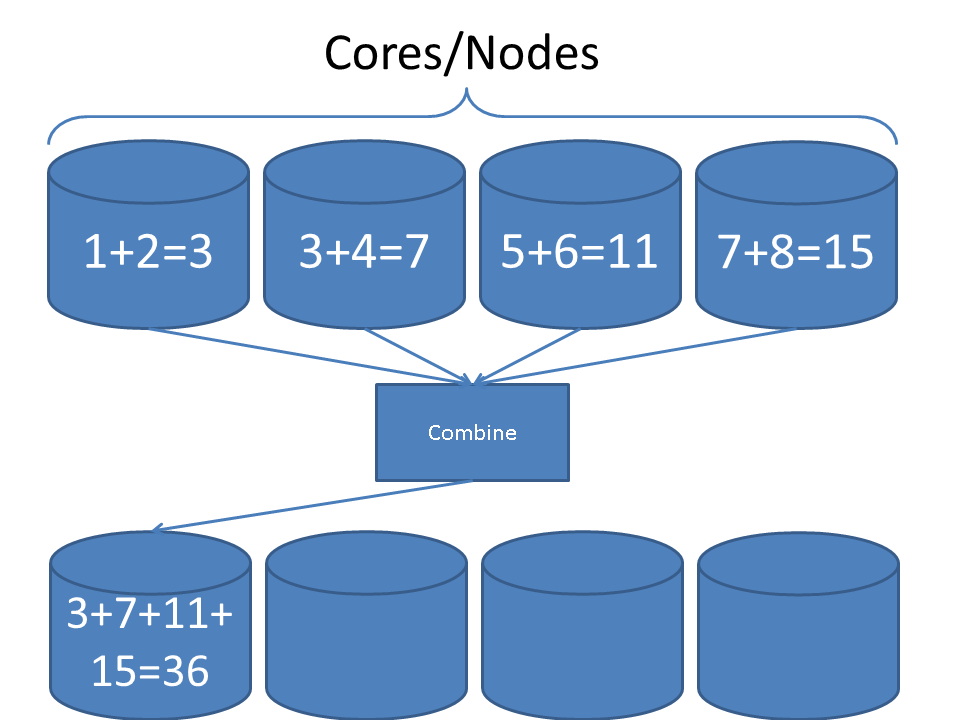
\includegraphics[width=.975\textwidth]{../common/pics/parallelism_data}
%       \end{center}
%       \end{block}
%     \end{minipage}
%     \hspace{.15cm}
%     \begin{minipage}{.46\textwidth}
%     \begin{block}{\centering Task Parallelism}
%       \begin{center}
%       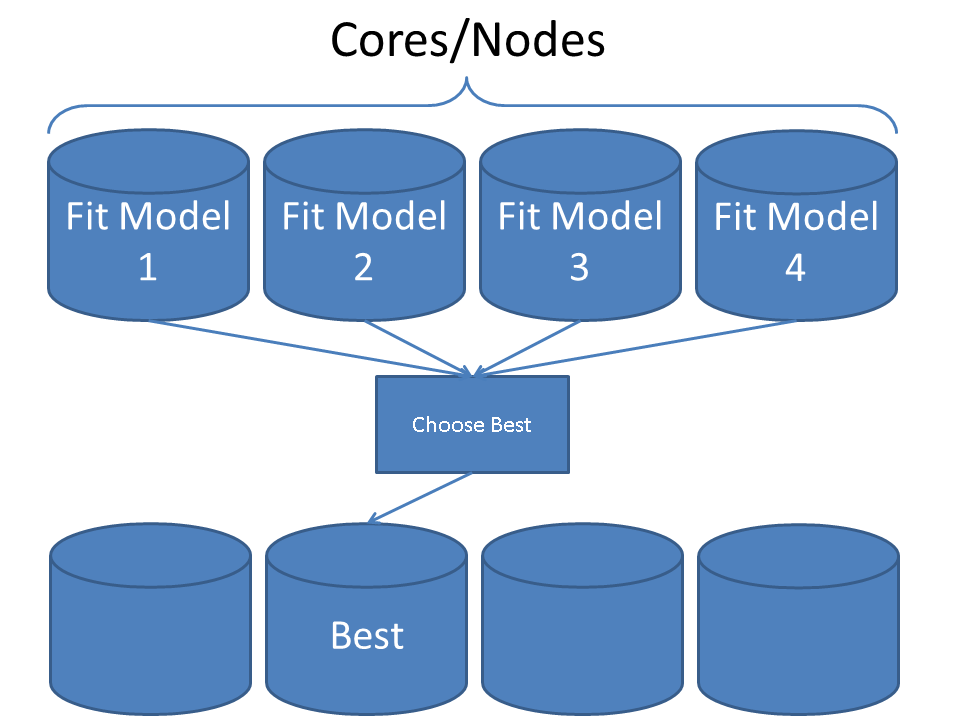
\includegraphics[width=.975\textwidth]{../common/pics/parallelism_task}
%       \end{center}
%       \end{block}
%     \end{minipage}
%     \end{center}
%   \end{block}
% \end{frame}




% \subsection{Common Terminology}


\begin{frame}
  \begin{block}{Difficulty in Parallelism}
  \begin{enumerate}[<+-|alert@+>]
    \item \emph{Implicit parallelism}:  Parallel details hidden from user
    \item \emph{Explicit parallelism}:  Some assembly required\dots
    \item \emph{Embarrassingly Parallel}:  Also called \emph{loosely coupled}.  
Obvious how to make parallel; lots of independence in computations.
    \item \emph{Tightly Coupled}:  Opposite of embarrassingly parallel; lots of 
dependence in computations.
  \end{enumerate}  
  \end{block}
\end{frame}


\begin{frame}
  \begin{block}{Speedup}
  \begin{itemize}
    \item \emph{Wallclock Time}:  Time of the clock on the wall from start to 
finish
    \item \emph{Speedup}:  unitless measure of improvement; more is better.
  \begin{align*}
   S_{n_1, n_2} =  \frac{\text{Run time for } n_1 \text{ cores}}{\text{Run time 
for } n_2 \text{ cores}}
  \end{align*}
  \begin{itemize}
    \item   $n_1$ is often taken to be 1
    \item In this case, comparing parallel algorithm to serial algorithm
  \end{itemize}
  \end{itemize}
  \end{block}
\end{frame}


\begin{frame}
   \begin{center}
    \begin{minipage}{.475\textwidth}
    \begin{block}{Good Speedup}
      \centering
      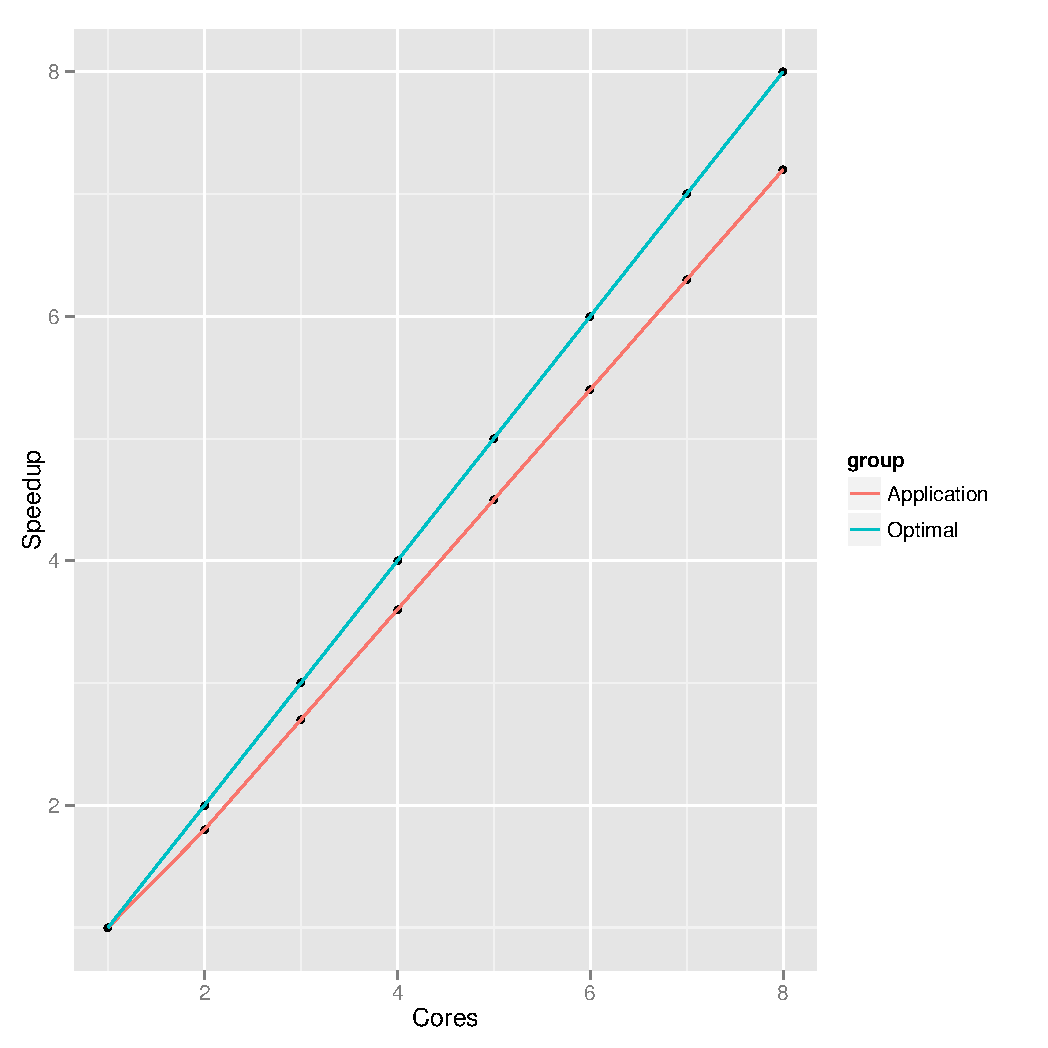
\includegraphics[width=.95\textwidth]{../common/pics/scale_good}
    \end{block}
    \end{minipage}
    \hspace{.1cm}
    \begin{minipage}{.475\textwidth}
    \begin{block}{Bad Speedup}
      \centering
      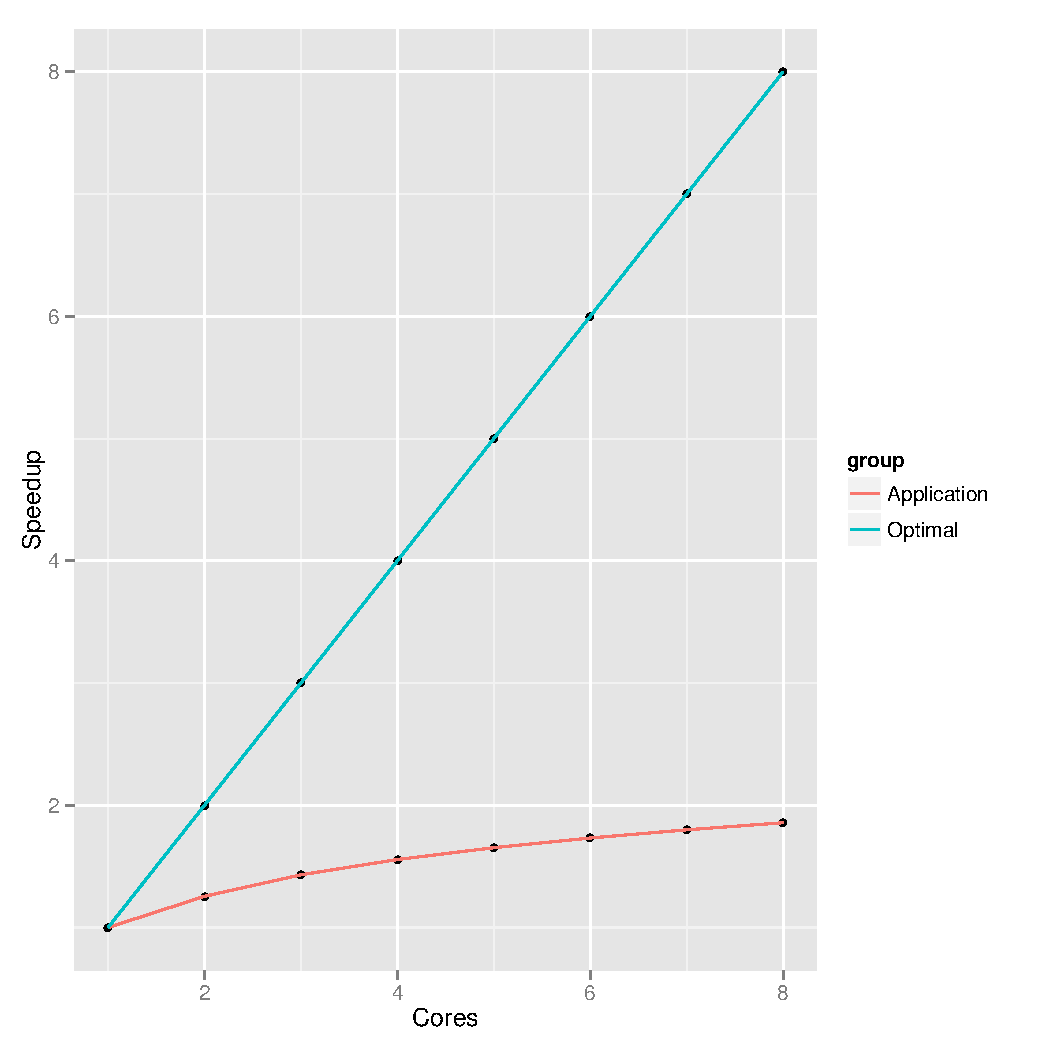
\includegraphics[width=.95\textwidth]{../common/pics/scale_bad}
    \end{block}
    \end{minipage}
    \end{center}
\end{frame}


\begin{frame}
  \begin{block}{Scalability and Benchmarking}
  \begin{enumerate}[<+-|alert@+>]
    \item \emph{Strong}:  Fixed \textbf{total} problem size.
    \item \emph{Weak}:  Fixed \textbf{local} (per processor) problem size.
  \end{enumerate}  
  \end{block}
\end{frame}


\begin{frame}
   \begin{center}
    \begin{minipage}{.475\textwidth}
    \begin{block}{Good Strong Scaling}
      \centering
      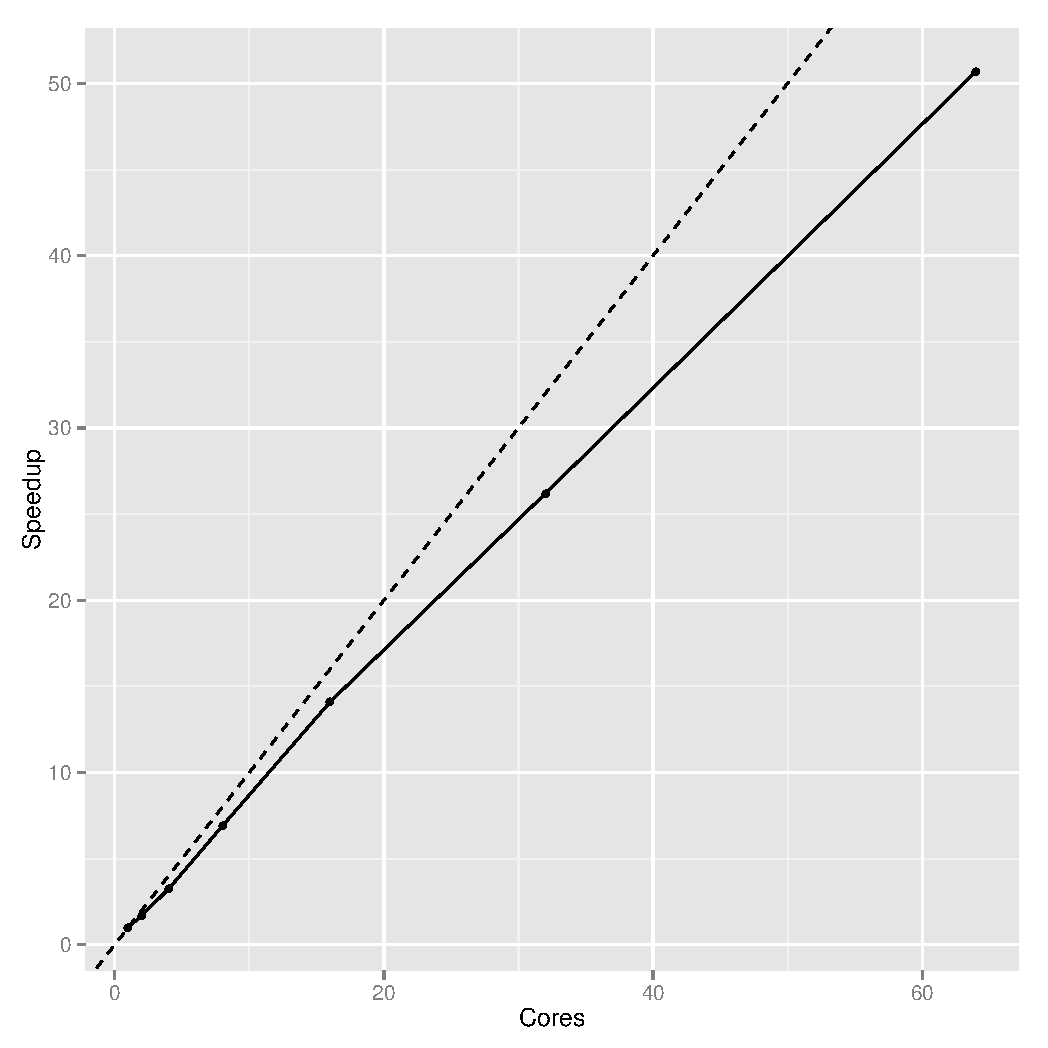
\includegraphics[width=.95\textwidth]{../common/pics/scaling_strong}
    \end{block}
    \end{minipage}
    \hspace{.1cm}
    \begin{minipage}{.475\textwidth}
    \begin{block}{Good Weak Scaling}
      \centering
      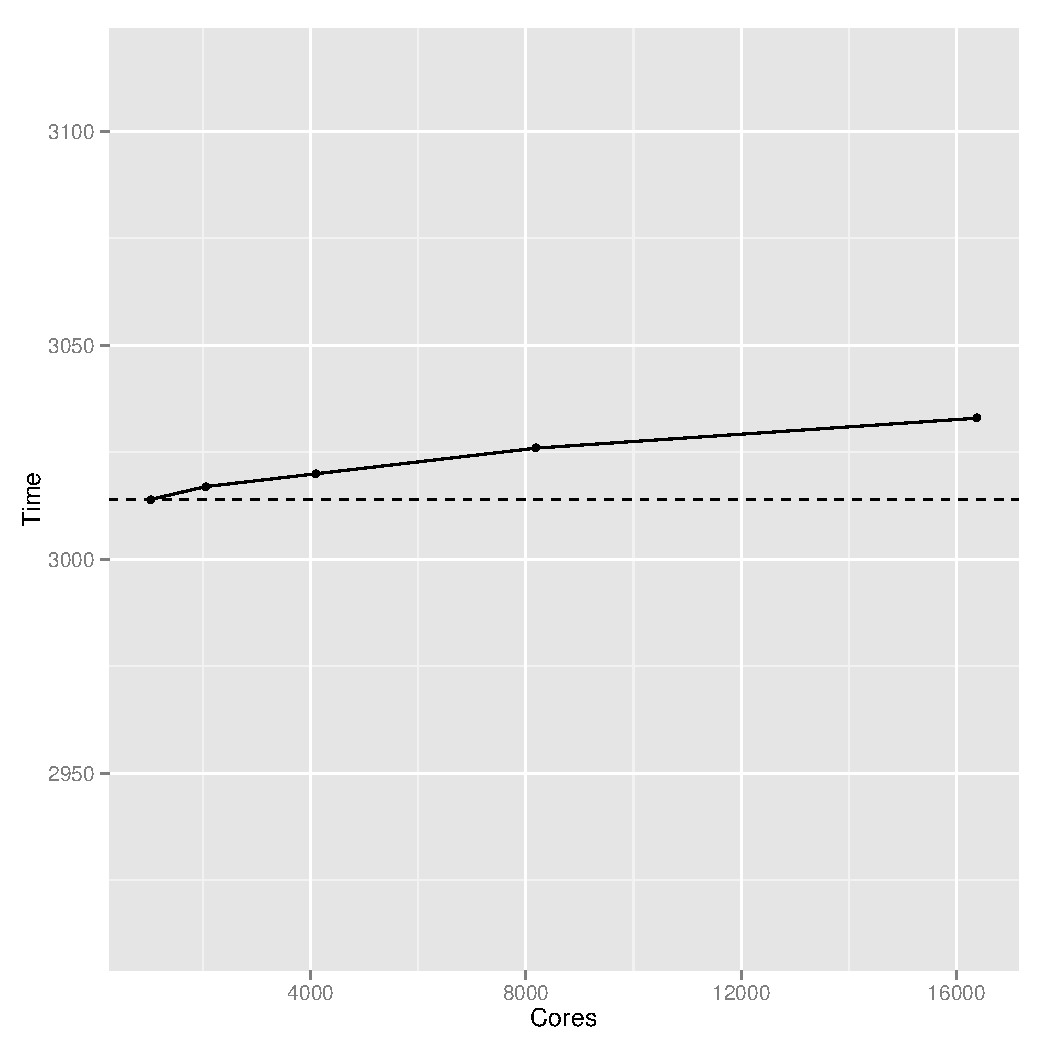
\includegraphics[width=.95\textwidth]{../common/pics/scaling_weak}
    \end{block}
    \end{minipage}
    \end{center}
\end{frame}



\begin{frame}
  \begin{block}{Shared and Distributed Memory Machines}
   \begin{center}
    \begin{minipage}{.475\textwidth}
    \begin{block}{Shared Memory}
     Direct access to read/change memory (one node) \vspace{.3cm} \ 
      \begin{center}
      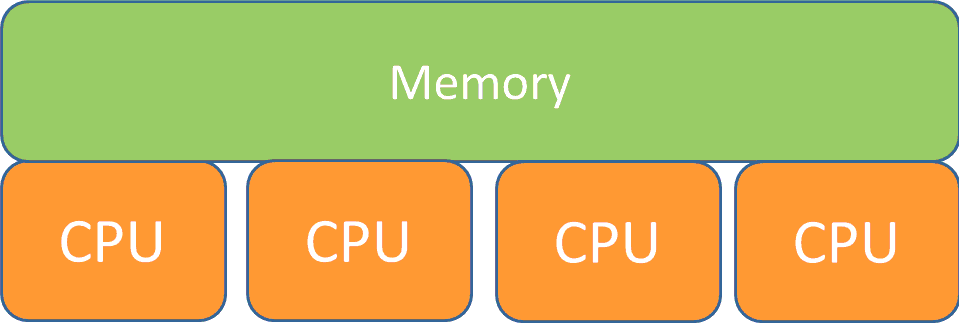
\includegraphics[width=.95\textwidth]{../common/pics/arch_shared}
      \end{center}
      \vspace{.3cm} \
    \end{block}
    \end{minipage}
    \hspace{.1cm}
    \begin{minipage}{.475\textwidth}
    \begin{block}{Distributed}
    No direct access to read/change memory (many nodes); requires communication
      \begin{center}
      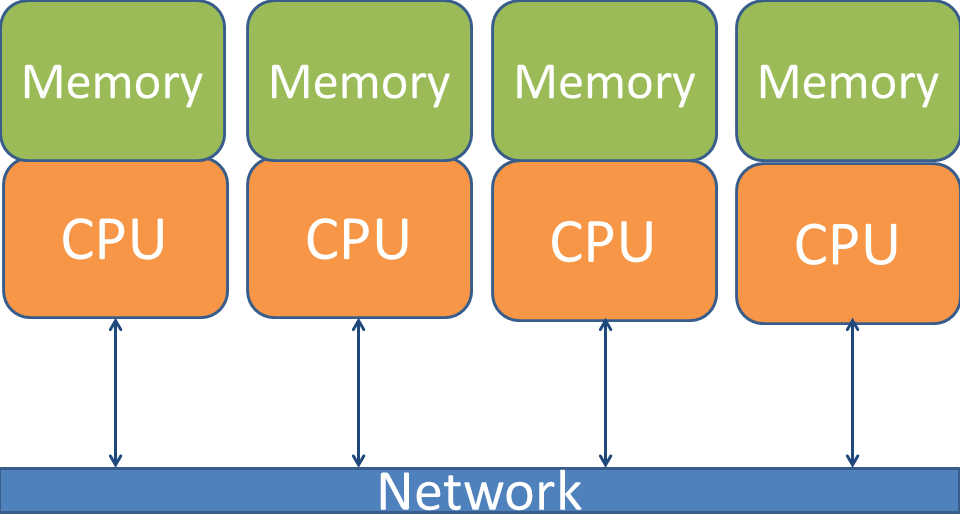
\includegraphics[width=.95\textwidth]{../common/pics/arch_distributed}
      \end{center}
    \end{block}
    \end{minipage}
    \end{center}
    \end{block}
\end{frame}


\begin{frame}
  \begin{block}{Shared and Distributed Memory Machines}
   \begin{center}
    \begin{minipage}[t]{.47\textwidth}
    \begin{block}{Shared Memory Machines}
    \begin{center}
    Thousands of cores\\[.2cm]
    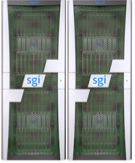
\includegraphics[scale=.65]{../common/pics/nautilus}\\
    {\tiny \emph{Nautilus}, University of Tennessee\\1024 cores \\4 TB RAM\\}
    \end{center}
    \end{block}
    \end{minipage}
    \hspace{.1cm}
    \begin{minipage}[t]{.47\textwidth}
    \begin{block}{Distributed Memory Machines}
    \begin{center}
    Hundreds of thousands of cores\\[.2cm]
    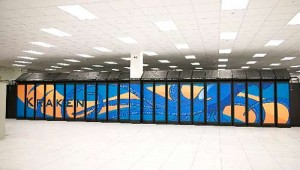
\includegraphics[width=.95\textwidth]{../common/pics/kraken}\\
    {\tiny \emph{Kraken}, University of Tennessee\\ 112,896 cores \\147 TB 
RAM\\}
    \end{center}
    \end{block}
    \end{minipage}
    \end{center}
    \end{block}
\end{frame}
